%! Author = Ian
%! Date = 12/4/2023

% Preamble
\documentclass[11pt]{article}

% Packages
\usepackage{amsmath}
\usepackage{graphics}
\usepackage{graphicx}

\title{Assignment 5 Writeup}
\author{Ian Chen}
\date{\today}

% Document
\begin{document}
    \maketitle

    \section{Face Detection}
    
    \begin{itemize}
    \item \textit{Face Classification}\newline
    I used the Viola-Jones algorithm, which uses AdaBoosting to train a strong classifier from a
    subset of Haar-like features. The algorithm is able to achieve a high detection rate while
    minimizing the number of false positives.
    % TODO: Answer

    \item \textit{Sliding Window + Human Classification}\newline
    I used the Viola-Jones algorithm along with the classifier cascade. The algorithm is also
    able to run in real time, as I used the classifier cascade to quickly reject non-face regions.\newline
    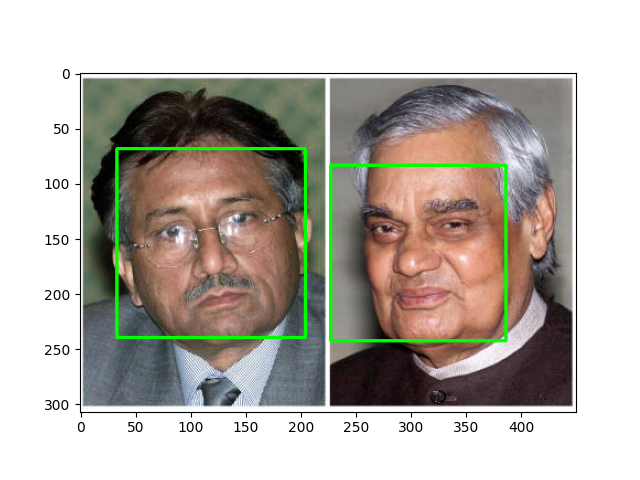
\includegraphics[width=0.3\textwidth]{Output Pictures/ex_1}
    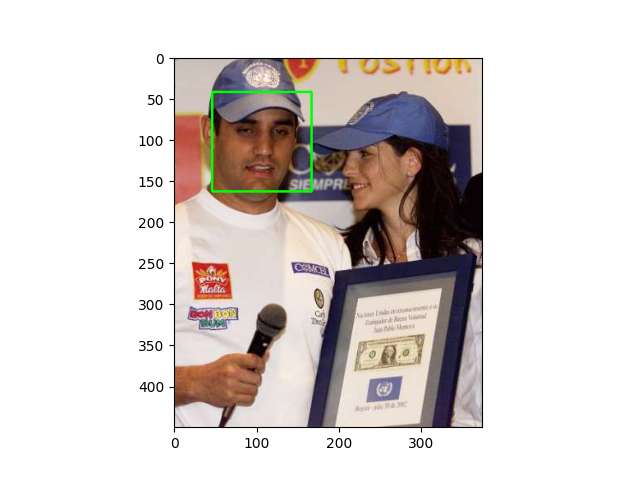
\includegraphics[width=0.3\textwidth]{Output Pictures/ex_2}
    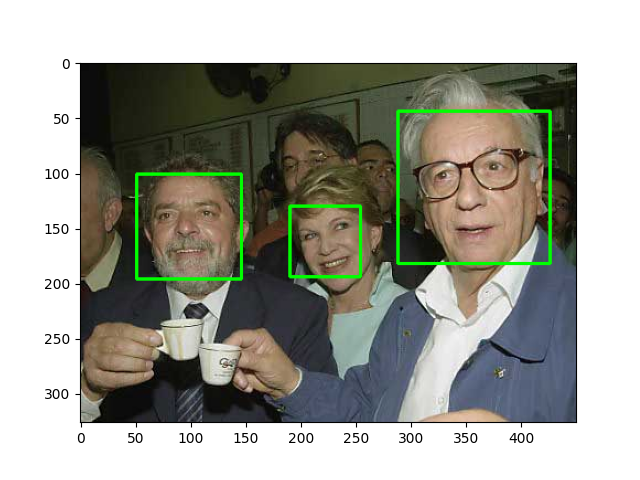
\includegraphics[width=0.3\textwidth]{Output Pictures/ex_3}

    % TODO: Answer

    \end{itemize}

    \section{Extra Credit}

    \begin{itemize}
    \item \textit{Object Detection}
    % TODO: Answer

    \item \textit{Running Time}
    % TODO: Answer

    \item \textit{Creative Ideas}
    % TODO: Answer

    \end{itemize}
\end{document}